\documentclass[11pt]{article}
\usepackage{../estilo-ejercicios}
\usepackage{wasysym}
\usetikzlibrary{automata,positioning}
\usepackage{mathdots}
\usepackage{listings}

\setlength{\parindent}{0em}
\setlength{\parskip}{1em}
\newcommand\tq{{\ \ /\ \ }}
\let \sii \Leftrightarrow
\let \luego \Rightarrow

\begin{document}
\begin{ejercicio}{1}
Definamos $F : \N^3\to \N$ por
$$F(x, e, t) = \text{valor de la variable }Y\text{ tras ejecutar el programa }e\text{ sobre }x\text{ durante }t\text{ pasos.}$$
Decimos que $x$ es un $F$-punto de $\varphi_e$ si $x \neq 0$ y para algún $t \in \N$, $F(x, e, t) = x$. Probar que:
\begin{enumerate}
\item $F$ es recursiva.
\item El conjunto $A = \{e \in \N : \varphi_e$ tiene un $F$-punto$\}$ es r.e.
\end{enumerate}
\end{ejercicio}
\begin{solucion}\
\begin{enumerate}
	\item $F(x,e,t)=(r(\texttt{di}(x,e,t))_1$, por lo que es primitiva recursiva.
	\item \[ A = \{ e \in \N : \exists x : F(x,e,t) = x \} \]
entonces:
\[ e \in A \sii \exists x \exists t : F(x,e,t) = x \]
Tomando $R(e,x) \sii F(x,e,t) = x$. Como $F$ es recursivo, $R$ es recursivo. Por el ejercicio 5.1 (consecuencia del teorema de proyección), $A$ es r.e.
\end{enumerate}
\end{solucion}

\newpage

\begin{ejercicio}{2}
Sea Prim $\subseteq \N$ el conjunto de los números primos. Pruébese que
\begin{enumerate}
\item El conjunto $A_1 = \{\#(P) : P$ es un programa $GOTO$ y rang$([\![P]\!]^{(1)})\subseteq$Prim$\}$ NO es un conjunto recursivo.
\item El conjunto $A_2 = \{e \in \N : \varphi_e(e)\in$Prim$\}$ es r.e. pero NO es recursivo.
\item El siguiente conjunto NO es r.e.
$$A_3 = \{e \in \N : (\forall x) [\varphi_e(x + e)\uparrow\lor \varphi_e(x)\uparrow \lor(\varphi_e(x + e)\downarrow \land \varphi_e(x)\downarrow \land \varphi_e(x + e) \neq \varphi_e(x))]\}$$
(Indicación: Utilícese el teorema del complemento y el teorema de recursión).
\end{enumerate}
\end{ejercicio}
\begin{solucion}\
\begin{enumerate}
	\item Sea
	\[  Γ = \{g \in \mathcal{P}^{(1)} : rang(g) \subseteq \text{Prim}\} \]
	Vemos que $Γ \neq \emptyset$ con el programa constante $2$ y vemos que $Γ \neq \mathcal{P}^{(1)}$ con el programa constante $1$. Entonces $A_1 = I_Γ$ es no recursivo por el teorema de Rice.
	
	\item Sea $\Gamma=\{ \varphi_e\in\mathcal{P}: \varphi_e(e)\in$Prim$\}$. Podemos usar las mismas funciones del apartado anterior, ya que al ser constantes sobre sus códigos dan los mismos resultados para probar por el teorema de Rice que $I_{\Gamma}=A_2$ no es recursivo.
	
	Para ver que es recursivamente enumerable vamos a ver que $\mathcal{K}$ es reducible a $A_2$. Sea $\mathcal{C}_3$ la función constantemente 3. Entonces $e\in\mathcal{K}\Leftrightarrow \mathcal{C}_3(e)\in A_2$. Como sabemos que $\mathcal{K}$ es r.e., entonces también lo es $A_2$. 
	
	\item Consideremos el complementario $\overline{A}_3$. Se va a probar que es r.e. y no recursivo, de modo que por el teorema del complemento, $A_3$ no puede ser r.e. Así pues, 
\begin{gather*}
e\in\overline{A}_2\sii (\exists x)[\varphi_e(x+e)\downarrow\land\varphi_e(x)\downarrow\land(\varphi_e(x+e)\uparrow\lor\varphi_e(x)\uparrow\lor \varphi_e(x+e)=\varphi_e(x))]\sii\\
\sii (\exists x)[\varphi_e(x+e)\downarrow\land\varphi_e(x)\downarrow\land\varphi_e(x+e)=\varphi_e(x))]
\end{gather*}
Sea ahora $g(u,v)=\mathcal{U}(v,u)$ recursiva, por el teorema de recursión existe $e$ tal que $\varphi_e(x)=g(e,x)=\mathcal{U}(x,e)$. En particular también $\varphi_e(x+e)=g(e,x+e)=\mathcal{U}(x+e,e)$. Sustituyendo esto en el predicado anterior deducimos que es recursivamente enumerable por ser un existencial sobre conjunciones de predicados r.e., y no recursivo (pues interviene el problema de la parada).
\end{enumerate}
\end{solucion}

\newpage
\begin{ejercicio}{3}
\[ 
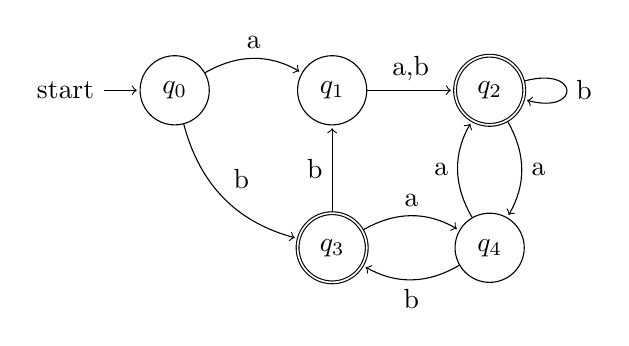
\begin{tikzpicture}[shorten >=1pt,node distance=2cm,on grid,auto] 
   \node[state,initial] (q_0)   {$q_0$}; 
   \node[state] (q_1) [right=of q_0] {$q_1$};
   \node[state,accepting] (q_2) [right=of q_1] {$q_2$};
   \node[state,accepting] (q_3) [below=of q_1] {$q_3$};
   \node[state] (q_4) [right=of q_3] {$q_4$};
    \path[->] 
    (q_0) edge [bend left] node {a} (q_1)
          edge [bend right] node {b} (q_3)
    (q_1) edge node {a,b} (q_2)
    (q_2) edge [bend left] node {a} (q_4)
          edge [loop right] node {b} ()
    (q_3) edge [bend left] node {a} (q_4)
          edge node {b} (q_1)
    (q_4) edge [bend left] node {b} (q_3)
          edge [bend left] node {a} (q_2);
\end{tikzpicture} \]
\end{ejercicio}
\begin{solucion}

\[ 
\begin{tikzpicture}[shorten >=1pt,node distance=2cm,on grid,auto] 
   \node[state,initial] (q_0)   {$q_0$}; 
   \node[state] (q_1) [right=of q_0] {$q_1$};
   \node[state] (q_2) [right=of q_1] {$q_2$};
   \node[state] (q_3) [below=of q_1] {$q_3$};
   \node[state] (q_4) [right=of q_3] {$q_4$};
   \node[state,accepting] (q_A) [below right=of q_4] {$q_A$};
    \path[->] 
    (q_0) edge [bend left] node {a} (q_1)
          edge [bend right] node {b} (q_3)
    (q_1) edge node {a+b} (q_2)
    (q_2) edge [bend left] node {a} (q_4)
          edge [loop right] node {b} ()
          edge [bend left] node {ϵ} (q_A)
    (q_3) edge [bend left] node {a} (q_4)
          edge node {b} (q_1)
          edge [bend right] node {ϵ} (q_A)
    (q_4) edge [bend left] node {b} (q_3)
          edge [bend left] node {a} (q_2);
\end{tikzpicture} \]
\[ 
\begin{tikzpicture}[shorten >=1pt,node distance=2cm,on grid,auto] 
   \node[state,initial] (q_0)   {$q_0$};
   \node[state] (q_2) [right=of q_1] {$q_2$};
   \node[state] (q_3) [below=of q_1] {$q_3$};
   \node[state] (q_4) [right=of q_3] {$q_4$};
   \node[state,accepting] (q_A) [below right=of q_4] {$q_A$};
    \path[->] 
    (q_0) edge [bend left] node {a(a+b)} (q_2)
          edge [bend right] node {b} (q_3)
    (q_2) edge [bend left] node {a} (q_4)
          edge [loop right] node {b} ()
          edge [bend left] node {ϵ} (q_A)
    (q_3) edge [bend left] node {a} (q_4)
          edge [bend left] node {b(a+b)} (q_2)
          edge [bend right] node {ϵ} (q_A)
    (q_4) edge [bend left] node {b} (q_3)
          edge [bend left] node {a} (q_2);
\end{tikzpicture} \]
\[ 
\begin{tikzpicture}[shorten >=1pt,node distance=4cm,on grid,auto] 
   \node[state,initial] (q_0)   {$q_0$};
   \node[state] (q_3) [below left=of q_0] {$q_3$};
   \node[state] (q_4) [below right=of q_3] {$q_4$};
   \node[state,accepting] (q_A) [right=of q_0] {$q_A$};
    \path[->] 
    (q_0) edge node {$a(a+b)(b)^*$} (q_A)
          edge [bend right] node {b} (q_3)
          edge [bend left] node {$a(a+b)b^*a$} (q_4)
    (q_3) edge node [pos=0.1,sloped] {$a+b(a+b)b^*a$} (q_4)
          edge node [sloped] {$ϵ+b(a+b)b^*$} (q_A)
    (q_4) edge [bend left] node {b} (q_3)
          edge [loop below] node {$ab^*a$} ()
          edge [bend right] node [below=0.3] {$ab^*$} (q_A);
\end{tikzpicture} \]

\[ 
\begin{tikzpicture}[shorten >=1pt,node distance=4.5cm,on grid,auto] 
   \node[state,initial] (q_0)   {$q_0$};
   \node[state] (q_4) [below right=of q_0] {$q_4$};
   \node[state,accepting] (q_A) [above right=of q_4] {$q_A$};
    \path[->] 
    (q_0) edge node {$a(a+b)b^*+b(ϵ+b(a+b)b^*)$} (q_A)
          edge [bend right] node [left] {$a(a+b)b^*a+b(a+b(a+b)b^*a)$} (q_4)
    (q_4) edge [loop below] node {$ab^*a$} ()
          edge [bend right] node [right] {$ab^*+b(ϵ+b(a+b)b^*$} (q_A);
\end{tikzpicture} \]
Expresión regular:
\[ a(a+b)b^*+b(ϵ+b(a+b)b^*)+(a(a+b)b^*a+b(a+b(a+b)b^*a)(ab^*a)^*(ab^*+b(ϵ+b(a+b)b^*)\]
Quitando las $ϵ$:
\[ a(a+b)b^*+b+bb(a+b)b^*+(a(a+b)b^*a+b(a+b(a+b)b^*a)(ab^*a)^*(ab^*+b+bb(a+b)b^*)\]
\end{solucion}
\end{document}
